%Copyright (c) 2017 Davide Quattrocchi All Rights Reserved.
\documentclass[a4paper,10pt]{report}
\usepackage[italian]{babel}
\usepackage[utf8]{inputenc}
\usepackage{graphicx, floatflt, eso-pic, svg, listings, multicol, enumitem}

\definecolor{bluekeywords}{rgb}{0,0,1}
\definecolor{greencomments}{rgb}{0,0.5,0}
\definecolor{redstrings}{rgb}{0.64,0.08,0.08}
\definecolor{xmlcomments}{rgb}{0.5,0.5,0.5}
\definecolor{types}{rgb}{0.17,0.57,0.68}

\lstset{%
	language=[Sharp]C,
	tabsize=2,
	keepspaces=true,
	captionpos=t,
	numbers=left,
	numberstyle=\tiny,
	frame=lines,
	showspaces=false,
	showtabs=false,
	breaklines=true,
	showstringspaces=false,
	breakatwhitespace=true,
	escapeinside={(*@}{@*)},
	commentstyle=\color{greencomments},
	morekeywords={partial, var, value, get, set},
	keywordstyle=\color{bluekeywords},
	stringstyle=\color{redstrings},
	basicstyle=\ttfamily\small,
	literate=%
	  {á}{{\'a}}1 {é}{{\'e}}1 {í}{{\'i}}1 {ó}{{\'o}}1 {ú}{{\'u}}1
	  {Á}{{\'A}}1 {É}{{\'E}}1 {Í}{{\'I}}1 {Ó}{{\'O}}1 {Ú}{{\'U}}1
	  {à}{{\`a}}1 {è}{{\`e}}1 {ì}{{\`i}}1 {ò}{{\`o}}1 {ù}{{\`u}}1
	  {À}{{\`A}}1 {È}{{\'E}}1 {Ì}{{\`I}}1 {Ò}{{\`O}}1 {Ù}{{\`U}}1
	  {ä}{{\"a}}1 {ë}{{\"e}}1 {ï}{{\"i}}1 {ö}{{\"o}}1 {ü}{{\"u}}1
	  {Ä}{{\"A}}1 {Ë}{{\"E}}1 {Ï}{{\"I}}1 {Ö}{{\"O}}1 {Ü}{{\"U}}1
	  {â}{{\^a}}1 {ê}{{\^e}}1 {î}{{\^i}}1 {ô}{{\^o}}1 {û}{{\^u}}1
	  {Â}{{\^A}}1 {Ê}{{\^E}}1 {Î}{{\^I}}1 {Ô}{{\^O}}1 {Û}{{\^U}}1
	  {œ}{{\oe}}1 {Œ}{{\OE}}1 {æ}{{\ae}}1 {Æ}{{\AE}}1 {ß}{{\ss}}1
	  {ű}{{\H{u}}}1 {Ű}{{\H{U}}}1 {ő}{{\H{o}}}1 {Ő}{{\H{O}}}1
	  {ç}{{\c c}}1 {Ç}{{\c C}}1 {ø}{{\o}}1 {å}{{\r a}}1 {Å}{{\r A}}1
	  {€}{{\euro}}1 {£}{{\pounds}}1 {«}{{\guillemotleft}}1
		{»}{{\guillemotright}}1 {ñ}{{\~n}}1 {Ñ}{{\~N}}1,
}
\addto\captionsitalian{%
	\renewcommand{\lstlistingname}{Codice}}
\addto\captionsitalian{%
	\renewcommand{\lstlistlistingname}{Codici sorgente}}

\frenchspacing
\makeatletter\patchcmd{\l@chapter}{1.0em}{0.1em}{}{}\makeatother
\makeatletter\@addtoreset{chapter}{part}\makeatother

\begin{document}
\begin{titlepage}
	\centering
	\vfill
	{\huge\bfseries N2L - Need 2 Log\par}
  \vspace{1cm}
  {\scshape\large\itshape Programma di utility per lo storage di credenziali personali.\par}
	\vspace{0.5cm}
  {\scshape\large Relazione del progetto di P.O.I.S.\par}
	\vspace{2cm}
	{\Large\itshape Davide Quattrocchi\par}
  {\large MATRICOLA: 273654\par}
	{\itshape d.quattrocchi@campus.uniurb.it\par}
	\vfill
  {\large A.A.:2016/17\par}
	\vspace{0.2cm}
	Professore: ~Edoardo \textsc{Bontà}\par
	\vspace{1.0cm}
	~Università degli Studi di Urbino \textsc{"Carlo Bo"}\par
	\vfill
  \vspace{0.5cm}
  Questo documento è stato preparato con \LaTeX.
  \end{titlepage}
\newpage
\tableofcontents
\newpage
\lstlistoflistings
\newpage
\chapter{Specifica del problema}
		Si vuole realizzare un sistema che dia la possibilità di salvare in modo
			sicuro gli account posseduti dall'utilizzatore in modo tale che egli non
			debba ricordare	ogni singola credenziale, username o password personale.\\
		Per poter rispettare suddetta specifica, il sistema dovrà possedere tali
		 	caratteristiche e comportamenti:
		\begin{itemize}
			\item Tutti i dati sensibili forniti dall'utente dovranno essere salvati
				all'interno di un database criptato.
			\item L'accesso al sistema e ai dati deve essere permesso solo dopo
				l'immissione e la verifica di una password, conservata in modo sicuro.
			\item Il sistema deve dare la possibilità di modificare ed eliminare
				i dati presenti nel database.
			\item Il sistema deve permettere di cambiare le impostazioni dell'applicazione,
				tra cui anche la password di accesso.
			\end{itemize}
\newpage
\chapter{Specifica dei requisiti}
	Osservando la specifica del problema risulta evidente quanto l’applicazione
		debba possedere efficienti sistemi di sicurezza, per preservare i dati
		dell’utilizzatore da un eventuale attacco informatico sui dati.\vfill
		In particolare, si è deciso di proteggere le informazioni che l’utente affida
		al sistema utilizzando questi metodi:\vfill
		\begin{itemize}
				\item La password di accesso al programma non verrà conservata in chiaro
					tra le impostazioni della applicazione, ma ne verrà conservato l'hash
					solo in fase di esecuzione,	calcolato tramite una apposita funzione
					crittografica di hash (i.e.: SHA-256).
				\item L'hash in questione verrà utilizzato come chiave di accesso e
					de/criptazione del database: così facendo, ci si affiderà al sistema
					di gestione della base di dati per accedere alle informazioni sicuramente.
				\item	L’applicazione può permettere di cambiare la password di accesso
					al sistema da parte dell’utente, così che l’utilizzatore riduca le
					probabilità che un attaccante riesca a sorpassare i	sistemi di
					sicurezza tramite attacchi basati su associazioni e confronti
					(bruteforcing, dictionary attack, rainbow tables attack, ecc).
			\end{itemize}
  \section{Organizzazione dell'applicativo}
    Si è deciso di separare, tramite la creazione di una DLL, il sistema di
			gestione dei dati dalla interfaccia utente, in modo tale che il sistema
			sia concettualmente più ordinato e che siano più facilmente implementabili
			futuri miglioramenti e aggiornamenti del programma.\\
			Si è dunque deciso di creare uno strato di comunicazione tra il DBMS
			scelto per lo storage dei dati e la applicazione che implementa la DLL,
			in modo tale da evitare che, con successive modifiche, le differenti
			versioni rischino di effettuare dei {\itshape breaking changes}.
  \section{Diagramma e descrizione dei casi d'uso}
    Di seguito vengono riportati i casi d’uso della applicazione basata su GUI,
			implementata tramite Windows Forms, per comprendere al meglio le
			funzionalità dell’applicativo.\\
			\begin{figure}[!h]
				\centering
				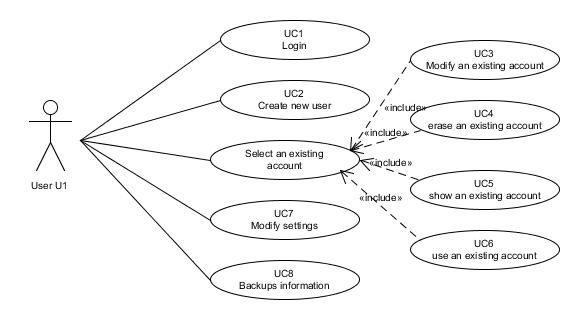
\includegraphics[width = \textwidth]{immagini/USE_CASE_DIAGRAM-UMLet2.jpg}
				\caption{Diagramma dei casi d'uso tramite GUI da parte dell'utente}
				\end{figure}
			Vengono riportati anche tutti i template dei casi d'uso sopra descritti.\\
			Poiché il processo di sviluppo utilizzato {\itshape(sezione 4.1)}
			prevede lo sviluppo orientato ai test, non è necessario effettuare
			test black-box sulla libreria (durante lo sviluppo vengono creati test
			white-box che coprono tutti i possibili flussi d’esecuzione) ed è quindi
			superfluo descrivere i template dei casi d’uso della libreria.
			\begin{figure}[htbp]
				\centering
				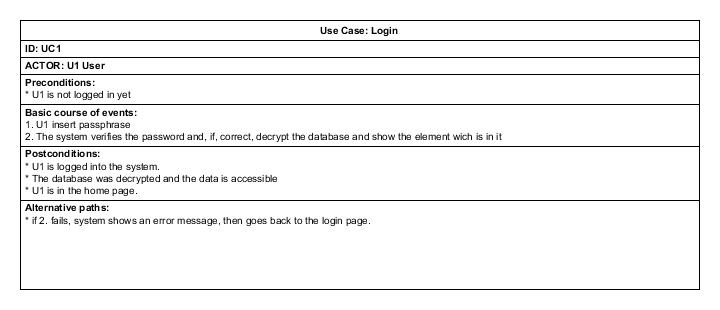
\includegraphics[width = \textwidth]{immagini/USE_CASE_TEMPLATE/UC01.jpg}
				\caption{Template relativo al caso d'uso UC1}
				\end{figure}
			\begin{figure}[htbp]
				\centering
				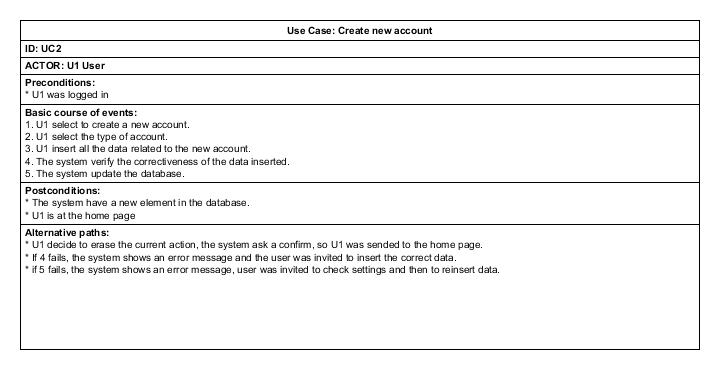
\includegraphics[width = \textwidth]{immagini/USE_CASE_TEMPLATE/UC02.jpg}
				\caption{Template relativo al caso d'uso UC2}
				\end{figure}
			\begin{figure}[htbp]
				\centering
				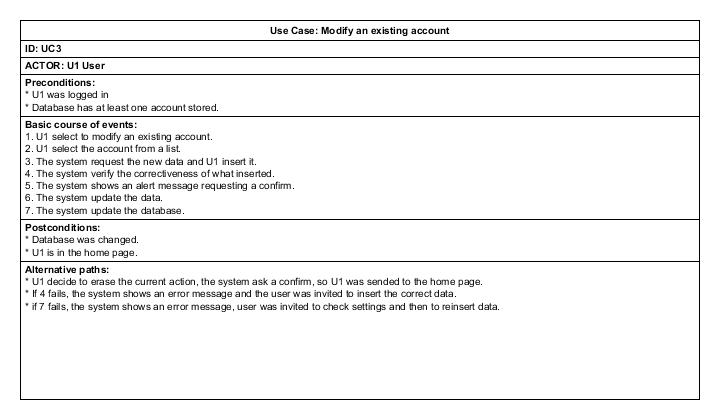
\includegraphics[width = \textwidth]{immagini/USE_CASE_TEMPLATE/UC03.jpg}
				\caption{Template relativo al caso d'uso UC3}
				\end{figure}
			\begin{figure}[htbp]
				\centering
				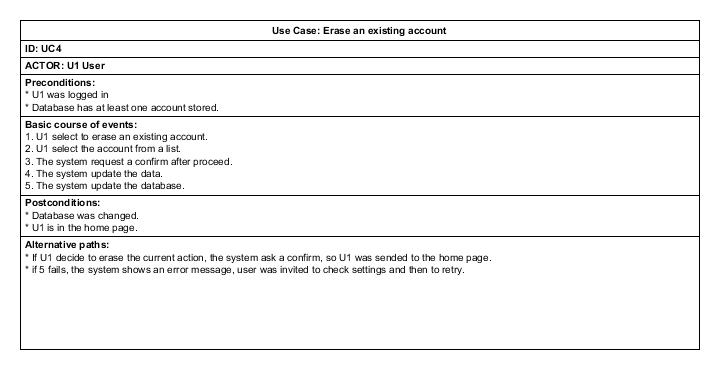
\includegraphics[width = \textwidth]{immagini/USE_CASE_TEMPLATE/UC04.jpg}
				\caption{Template relativo al caso d'uso UC4}
				\end{figure}
			\begin{figure}[htbp]
				\centering
				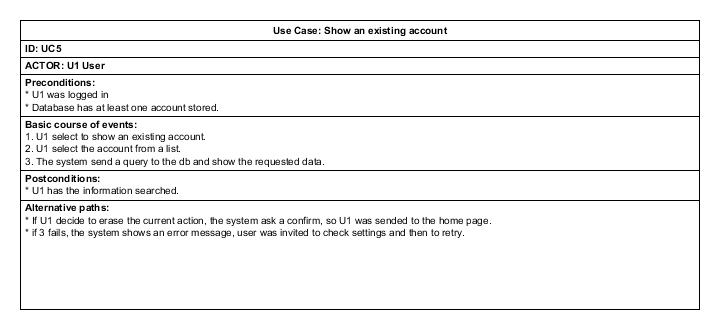
\includegraphics[width = \textwidth]{immagini/USE_CASE_TEMPLATE/UC05.jpg}
				\caption{Template relativo al caso d'uso UC5}
				\end{figure}
			\begin{figure}[htbp]
				\centering
				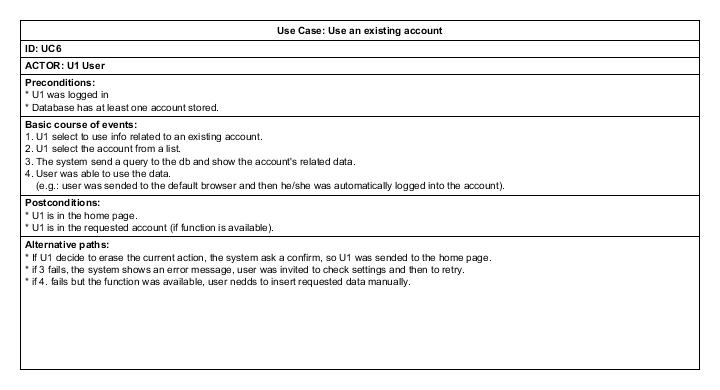
\includegraphics[width = \textwidth]{immagini/USE_CASE_TEMPLATE/UC06.jpg}
				\caption{Template relativo al caso d'uso UC6}
				\end{figure}
			\begin{figure}[htbp]
				\centering
				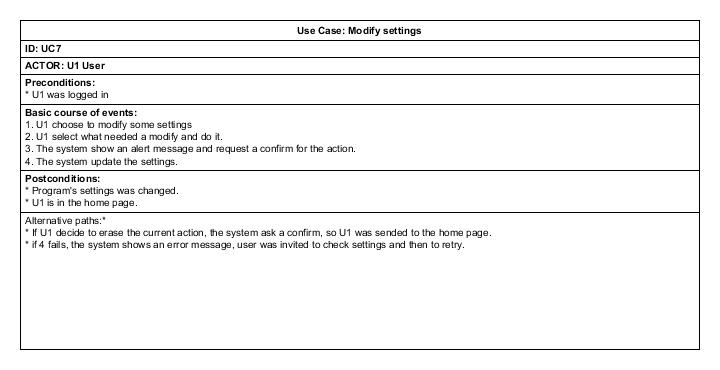
\includegraphics[width = \textwidth]{immagini/USE_CASE_TEMPLATE/UC07.jpg}
				\caption{Template relativo al caso d'uso UC7}
				\end{figure}
			\begin{figure}[htbp]
				\centering
				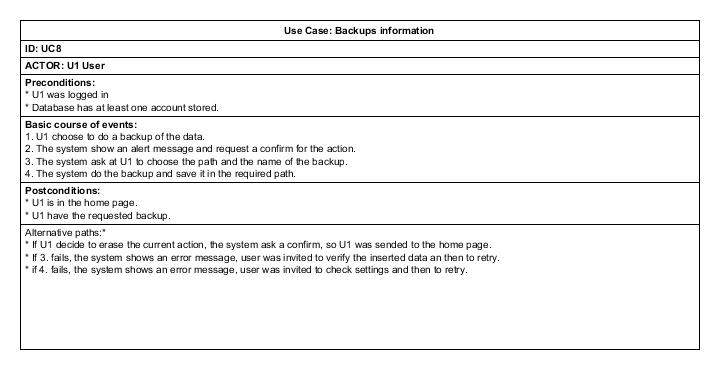
\includegraphics[width = \textwidth]{immagini/USE_CASE_TEMPLATE/UC08.jpg}
				\caption{Template relativo al caso d'uso UC8}
				\end{figure}
\newpage
\chapter{Analisi e progettazione}
	\section{Linguaggio di Programmazione}
		Per la realizzazione della interfaccia grafica e della libreria verrà
			utilizzato il linguaggio di programmazione C\# (C-sharp).\\
			Tale linguaggio è di tipo {\itshape multi paradigma}: la sua struttura e
			sintassi sono ispirati da vari linguaggi precedenti a questo per nascita,
			evolvendoli ripulendo il codice da simbolismi ed elementi decorativi.\\
			Il linguaggio opera all'interno del Framework {\itshape .NET}, che è una
			suite di prodotti di tecnologia di programmazione ad oggetti.
	\section{Ambiente di sviluppo}
		Per lo sviluppo dell'applicazione è stato scelto di utilizzare come IDE
			{\itshape Visual Studio Express 2017}: sviluppato da Microsoft
			(esattamente come il linguaggio di programmazione selezionato),
			funzionante su Sistemi Operativi Microsoft Windows, supporta
			perfettamente il linguaggio di programmazione scelto.
	\section{Database e DBMS}
		Per la memorizzazione dei dati si è scelto di utilizzare SQLite,
			per la sua semplicità d’utilizzo, la sua persistenza in locale
			e per la sua gestione ottimale.\\
			Infatti tutta la base di dati (tabelle, query, report etc..) è presente in
			un unico file, garantendo così la portabilità dei dati.\\
			Quando l’applicazione viene eseguita, si controlla se esiste un database
			dal nome "{\itshape DBN2L.sqlite3}" e se esiste si procede ad effettuare
			l’accesso; in caso contrario si crea.\\
			Il percorso del file è una sottodirectory della libreria, dove si trova
			cioè il file .dll necessario al funzionamento degli applicativi.\\
			La libreria è stata progettata per implementare, a livello concettuale,
			qualunque altro DBMS si voglia, dando anche la possibilità di affiancarli
			tra loro.
	\section{GUI}
		Per implementare le funzionalità offerte dal sistema e per rendere
			l'utilizzo di tali funzioni semplici per l'utente classico, si è deciso
			di creare una applicazione con interfaccia grafica.\\
			Tale GUI è stata realizzata tramite l'utilizzo delle classi delle
			Windows Forms del framework .NET.\\
			Tra le classi grafiche utilizzate nel programma troviamo le seguenti:
			\begin{itemize}
				\item {\itshape Form}: Rappresenta una finestra o una finestra di dialogo
					che compone l'interfaccia utente di un'applicazione.
				\item {\itshape MessageBox}: Visualizza una finestra di messaggio, nota
					anche come finestra di dialogo, che presenta un messaggio all'utente.\\
					Si tratta di una finestra modale, che impedisce altre azioni
					nell'applicazione fino alla sua chiusura.\\
					Un oggetto {\itshape System.Windows.Forms.MessageBox} può contenere
					testo, pulsanti e simboli che forniscono istruzioni e
					informazioni all'utente.
				\item {\itshape SaveFileDialog}: Richiede all'utente di selezionare un
					percorso per salvare un file.
				\item {\itshape PictureBox}: Rappresenta un controllo casella di
					immagine di Windows per la visualizzazione di un'immagine.
			\end{itemize}
			Sono stati introdotti in totale 7 Form:
			\begin{itemize}
				\item {\itshape DetailedInfo}: Form utile a mostrare all'utente tutte le
					informazioni relative ad un account selezionato tra quelli
					disponibili e/o a modificarlo.
				\item {\itshape FormAboutBox}: Form della finestra "informazioni su"
					relative alla applicazione.
				\item {\itshape FormCreate}: Form utile a creare un nuovo account da
				 	inserire nella lista di account esistenti.
				\item {\itshape FormFirstAccess}: Form utile a settare le impostazioni
					iniziali (username e password) prima della creazione del database.
				\item {\itshape FormLogin}: Form utile a permettere all'utente di
					accedere al sistema.
				\item {\itshape FormMainMenu}: Form principale della applicazione, dove
					vengono svolte le principali azioni.
				\item {\itshape FormOption}: Form utile a modificare le impostazioni
					necessarie per il corretto funzionamento della applicazione
					(username e password).
			\end{itemize}
	\newpage
	\section{Pattern usati}
		In fase di progettazione sono stati individuati dei problemi tipicamente
			ricorrenti, ai quali si è deciso di trovare soluzione tramite la
			implementazione dei design pattern.\\
			Nello specifico, si è ritenuto necessario dover utilizzare i seguenti:
		\subsection{Singleton}
			{\itshape Singleton} è un pattern creazionale basato su oggetti che
			risolve il problema di assicurare che per una classe esista un’unica
			istanza accessibile con semplicità, facendo in modo che sia la classe
			stessa ad istanziarsi.\\
			Singleton è applicabile quando:
			\begin{itemize}
				\item Deve esistere un’unica istanza di una classe accessibile
					da un riferimento noto a tutti gli utilizzatori;
				\item L’unica istanza deve essere estesa con sottoclassi e
					anch’esse devono ammettere un’unica istanza.
				\end{itemize}
			Per far funzionare correttamente il pattern, il costruttore della classe
			deve essere privato (nel caso in cui si debba verificare la prima
			precondizione) o protetto (nel caso in cui si debba verificare la seconda).\\
			L’implementazione di Singleton consiste nella creazione di un metodo pubblico
			e statico (in genere chiamato Instance) che restituisce il riferimento
			all’istanza, non accessibile direttamente dall’esterno, dell’oggetto
			(in genere contenuta nell’attributo privato \_instance), se il riferimento è
			nullo, invoca il costruttore prima di resituirlo.\\
			Questo pattern sarà utilizzato all'interno della classe Core.DBConnector.
			\begin{center}
				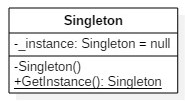
\includegraphics[scale=1]{immagini/Singleton.jpg}
				\end{center}
			\begin{figure}[!h]
					\caption{Diagramma UML del Design Pattern Singleton}
				\end{figure}
		\newpage
		\subsection{Template Method}
			{\itshape Template Method}è un pattern comportamentale basato su classi
				che  permette di definire la struttura di un algoritmo lasciando alle
				sottoclassi il compito di implementarne alcuni passi come preferiscono,
				personalizzando in queste il comportamento senza dover riscrivere più
				volte il codice in comune.\\
				Template Method è applicabile quando:
			\begin{itemize}
				\item si vuole implementare la parte comune di un algoritmo una
					volta sola, lasciando alle sottoclassi il compito di implementare il
					comportamento che può variare;
				\item il comportamento comune di più classi può essere inserito
					in una classe a parte per evitare di scrivere più volte
					lo stesso codice;
				\end{itemize}
			Questo pattern verrà utilizzato dalle classi Core.QueryCreator
			e Core.SQLiteQueryCreator.
			\begin{center}
				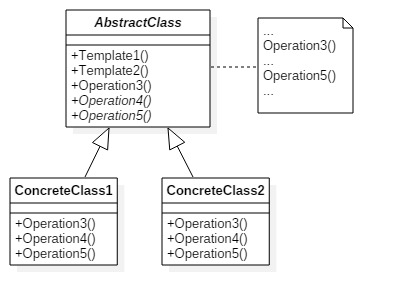
\includegraphics[scale=1]{immagini/TemplateMethod.jpg}
				\end{center}
			\begin{figure}[!h]
					\caption{Diagramma UML del Design Pattern Template Method}
				\end{figure}
		\newpage
		\subsection{Architettura n-tier}
			Una {\itshape architettura n-tier}, o {\itshape multi-tier}, è una
				architettura software in cui le varie funzionalità sono disaccoppiate a
				livello logico su vari livelli in comunicazione diretta tra loro solo
				tramite i livelli tra loro adiacenti mediante il modello client-server.
				Un esempio classico di queste architetture è quello delle applicazioni
				web, queste infatti hanno 3 livelli logici separati tra loro che sono:
				\begin{enumerate}
					\item logica di presentazione
					\item elaborazione dei processi
					\item persistenza dei dati
				\end{enumerate}
				Il livello 1 è in comunicazione solo con il livello 2,
				il livello 2 è in comunicazione con il livello 1 e il livello 3,
				il livello 3 è in comunicazione solo con il livello 2.\\
				Questa architettura viene utilizzata all'interno della soluzione
				associata a questo report, in quanto la libreria {\itshape Core} funge
				da intermediario tra la base di dati e un qualsiasi programma che voglia
				sfruttare tale libreria (in questo caso il nostro progetto con
				intefaccia grafica).
				\\\vspace{1cm}
				\begin{center}
					\Huge{
						{\itshape DBMS}
						{\longleftrightarrow}
						{\itshape N2L.Core}
						{\longleftrightarrow}
						{\itshape GUI}
						}
					\end{center}
	\newpage
	\section{Classi}
		Di seguito verranno forniti i diagrammi UML relativi ad ogni singola classe
		creata all'interno di ogni progetto, divisi per questi.
		\subsection{N2L.Core}
			Le classi che compongono la libreria DLL.
			\begin{itemize}
				\item[] {
					\begin{center}
						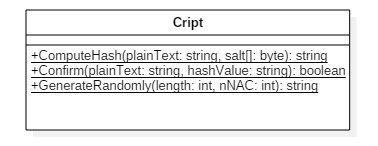
\includegraphics[scale=1]{immagini/Cript.jpg}
						\end{center}
					\begin{figure}[!h]
							\caption{Diagramma UML della classe Cript}
						\end{figure}}
				\item[] {
					\begin{center}
						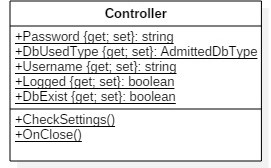
\includegraphics[scale=1]{immagini/Controller.jpg}
						\end{center}
					\begin{figure}[!h]
						\caption{Diagramma UML della classe Controller}
						\end{figure}}
				\item[] {
					\begin{center}
						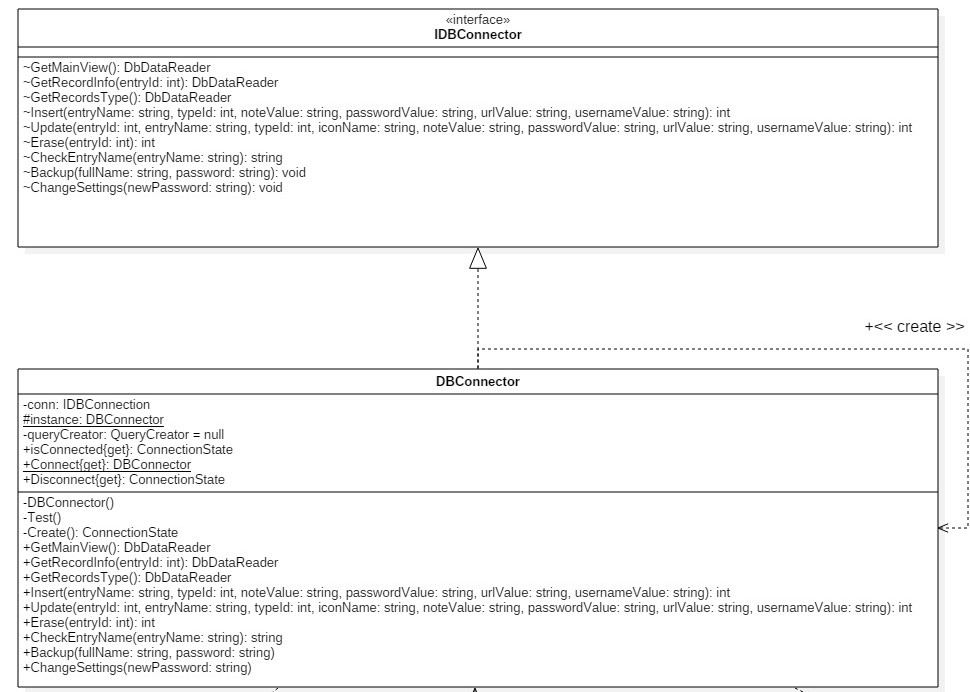
\includegraphics[width=\textwidth]{immagini/DBConnector.jpg}
						\end{center}
					\begin{figure}[!h]
							\caption{Diagramma UML della classe DBConnector e della sua interfaccia}
						\end{figure}}
				\item[] {
					\begin{center}
						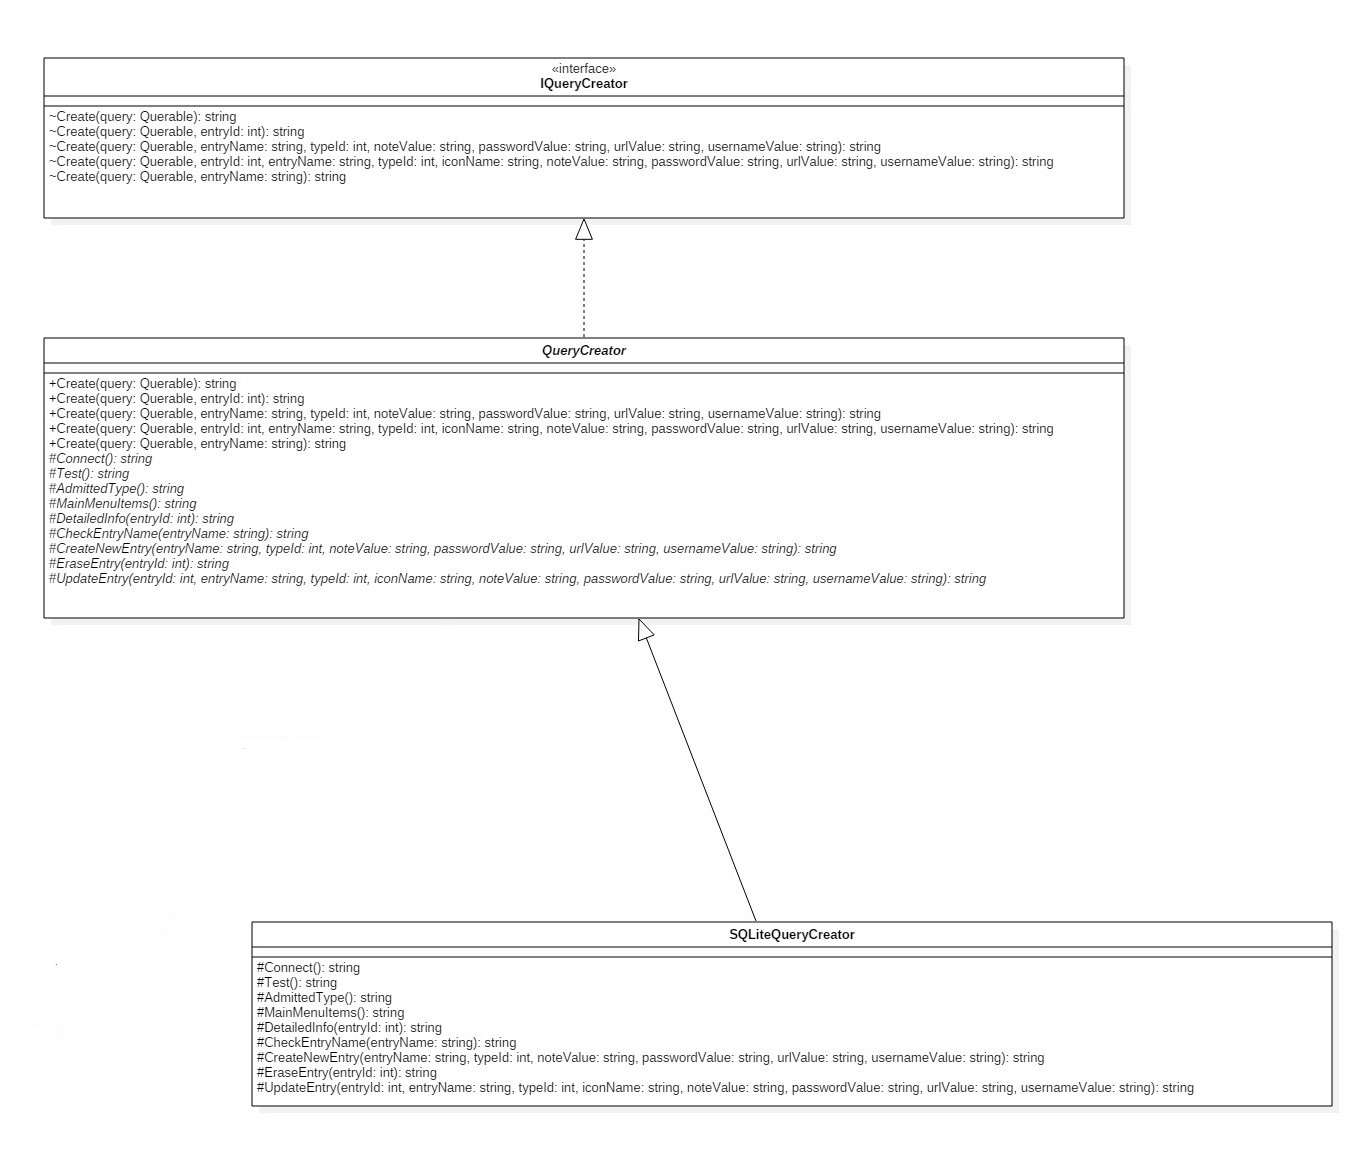
\includegraphics[width=\textwidth]{immagini/QueryCreator.jpg}
						\end{center}
					\begin{figure}[!h]
						\caption{Diagramma UML della classe QueryCreator, della sua interfaccia e di una sua implementazione}
						\end{figure}}
				\end{itemize}
		\newpage
		\subsection{N2L.Core.DataStruct}
			Le classi che compongono le strutture dati usate nella libreria.
			\begin{itemize}
				\item[] {
					\begin{center}
						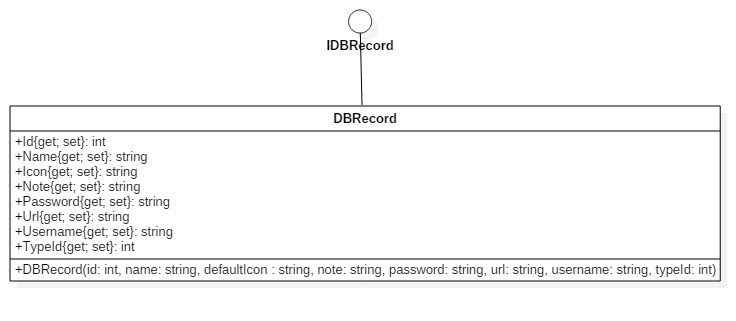
\includegraphics[width = \textwidth]{immagini/DBRecord.jpg}
						\end{center}
					\begin{figure}[!h]
						\caption{Diagramma UML della classe DBRecord e della sua interfaccia}
						\end{figure}}
				\item[] {
					\begin{center}
						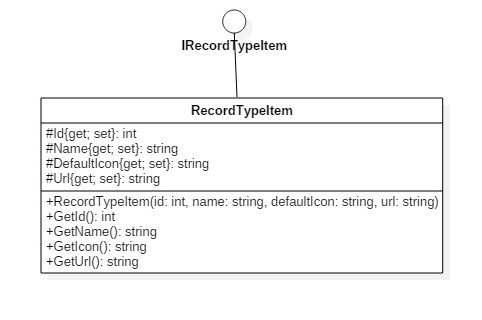
\includegraphics[width = \textwidth]{immagini/RecordTypeItem.jpg}
						\end{center}
					\begin{figure}[!htb]
					\caption{Diagramma UML della classe RecordTypeItem e della sua interfaccia}
					\end{figure}}
				\end{itemize}
		\newpage
		\subsection{N2L.DesktopFormsGUI}
			Le classi che compongono l'implementazione della GUI.
			\begin{itemize}
				\item[] {
					\begin{center}
						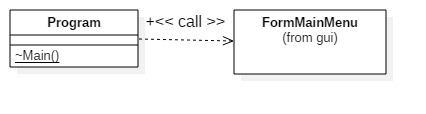
\includegraphics[width = \textwidth]{immagini/Program.jpg}
						\end{center}
					\begin{figure}[!h]
						\caption{Diagramma UML della classe Program}
						\end{figure}}
				\item[] {
					\begin{center}
						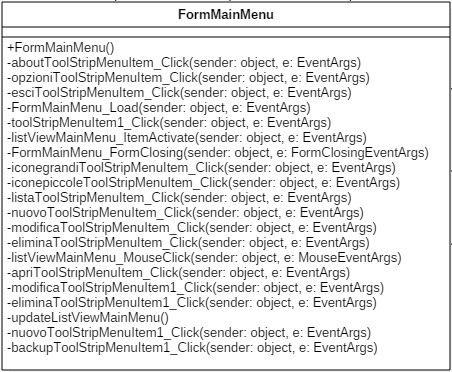
\includegraphics[width = \textwidth]{immagini/FormMainMenu.jpg}
						\end{center}
					\begin{figure}[!h]
						\caption{Diagramma UML della classe FormMainMenu}
						\end{figure}}
				\item[] {
					\begin{center}
						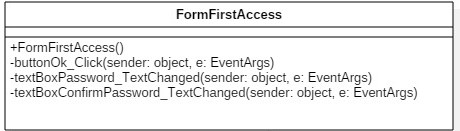
\includegraphics[width = \textwidth]{immagini/FormFirstAccess.jpg}
						\end{center}
					\begin{figure}[!h]
						\caption{Diagramma UML della classe FormFirstAccess}
						\end{figure}}
				\item[] {
					\begin{center}
						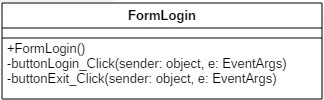
\includegraphics[scale=1]{immagini/FormLogin.jpg}
						\end{center}
					\begin{figure}[!h]
						\caption{Diagramma UML della classe FormLogin}
						\end{figure}}
				\item[] {
					\begin{center}
						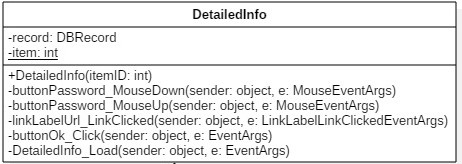
\includegraphics[width = \textwidth]{immagini/DetailedInfo.jpg}
						\end{center}
					\begin{figure}[!h]
						\caption{Diagramma UML della classe DetailedInfo}
						\end{figure}}
				\item[] {
					\begin{center}
						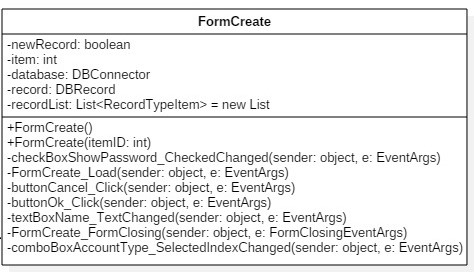
\includegraphics[width = \textwidth]{immagini/FormCreate.jpg}
						\end{center}
					\begin{figure}[!h]
						\caption{Diagramma UML della classe FormCreate}
						\end{figure}}
				\item[] {
					\begin{center}
						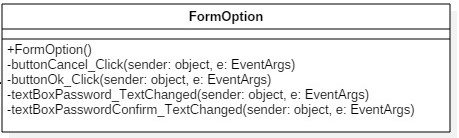
\includegraphics[width = \textwidth]{immagini/FormOption.jpg}
						\end{center}
					\begin{figure}[!h]
						\caption{Diagramma UML della classe FormOption}
						\end{figure}}
				\item[] {
					\begin{center}
						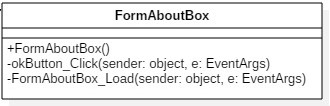
\includegraphics[scale=1]{immagini/FormAboutBox.jpg}
						\end{center}
					\begin{figure}[!h]
						\caption{Diagramma UML della classe FormAboutBox}
						\end{figure}}
				\end{itemize}
		\newpage
		\subsection{N2L.ConsoleTest}
			La classe che compone l'applicazione di test della DLL.
				\begin{itemize}
					\item[] {
						\begin{center}
							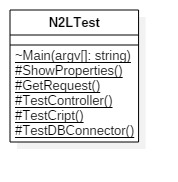
\includegraphics[scale=0.7]{immagini/N2LTestClasses.jpg}
							\end{center}
						\begin{figure}[!h]
							\caption{Diagramma UML della classe N2L.ConsoleTest.N2LTest}
							\end{figure}}
					\end{itemize}
		\newpage
		\subsection{Diagrammi delle classi completi}
			\begin{itemize}
				\item[] {
					\begin{center}
						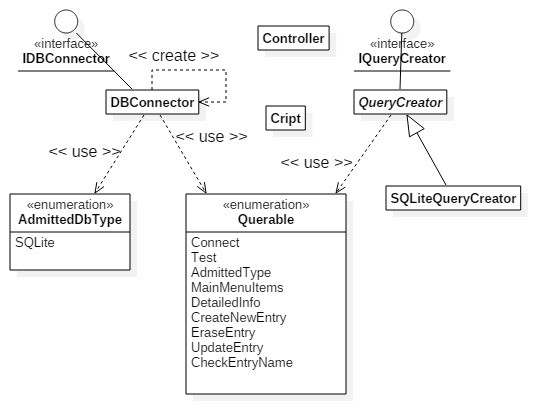
\includegraphics[width=\textwidth]{immagini/Core.jpg}
						\end{center}
					\begin{figure}[!h]
						\caption{Diagramma UML del namespace Core}
						\end{figure}}
				\item[] {
					\begin{center}
						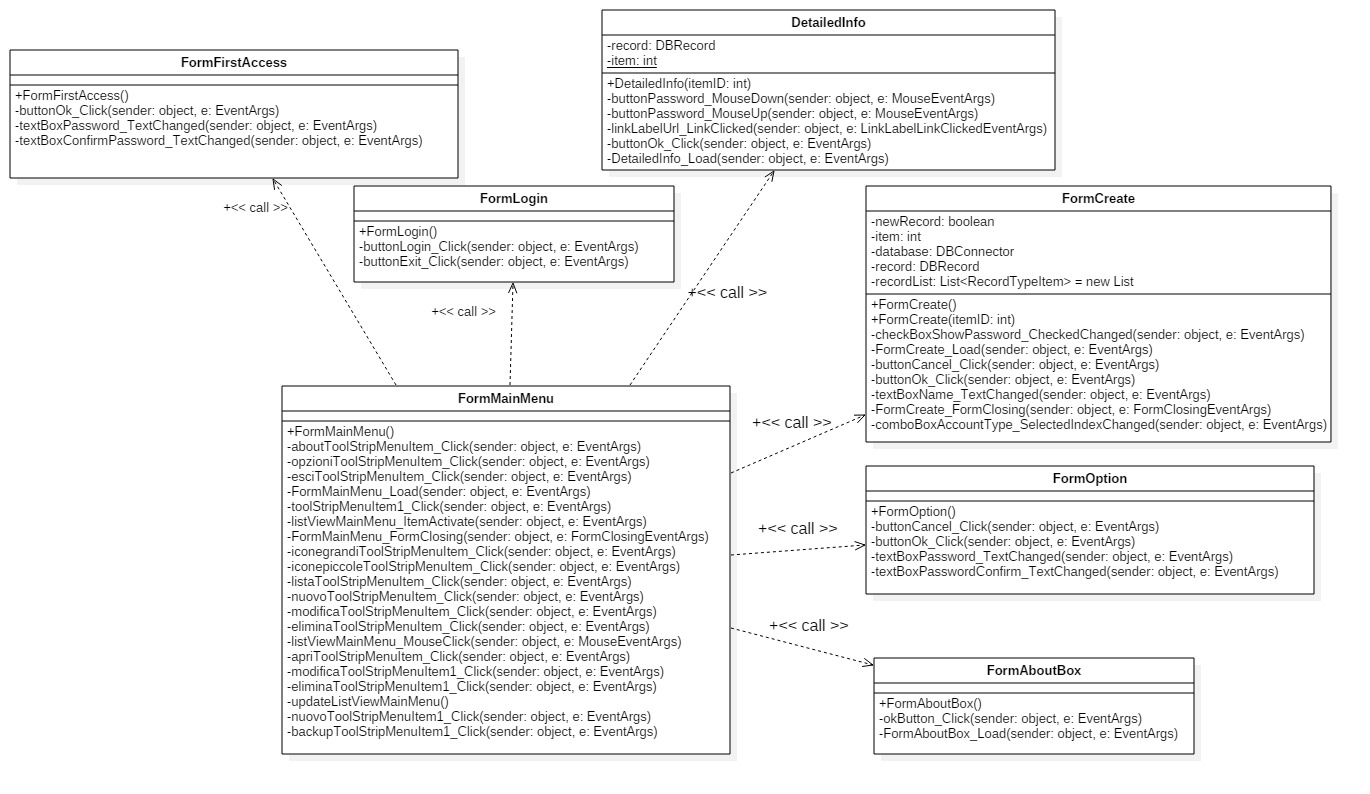
\includegraphics[width=\textwidth]{immagini/N2LDesktopFormsGUIguiClasses.jpg}
						\end{center}
					\begin{figure}[!h]
						\caption{Diagramma UML del namespace DesktopFormsGUI.gui}
						\end{figure}}
				\end{itemize}
\newpage
\chapter{Implementazione}
  \section{Processo di sviluppo}
    Un processo di sviluppo è un insieme di attività (principali e secondarie)
			atte a ottenere una migliore pianificazione e gestione durante lo
			sviluppo di software.\\
			Il processo di sviluppo utilizzato, visto che è presente un solo
			sviluppatore (situazione che obbliga ad escludere dunque le pratiche
			di pair programming e simili), è Extreme Programming (XP).\\
			Extreme Programming è un processo di sviluppo {\itshape agile}, ossia un
			processo che predilige pianificazione adattativa, sviluppo evolutivo,
			consegne anticipate, miglioramento continuo ed è in grado di rispondere
			ai cambiamenti in maniera rapida e flessibile.
	\section{Classi della libreria "{\scshape\itshape Core}"}
    Classi presenti:
		\begin{multicols}{2}
			\begin{itemize}
				\item Controller.cs
				\item Cript.cs
				\item DBConnector.cs
				\item IDBConnector.cs
				\item IQueryCreator.cs
				\item QueryCreator.cs
				\item SQLiteQueryCreator.cs
				\item DataStruct/IDBRecord.cs
				\item DataStruct/DbRecord.cs
				\item DataStruct/IRecordTypeItem.cs
				\item DataStruct/RecordTypeItem.cs
			\end{itemize}
			\end{multicols}
		\newpage
		\lstinputlisting[label=Controller, caption=Classe Controller.cs]{../Need2Log/Core/Controller.cs}
		\lstinputlisting[label=Cript, caption=Classe Cript.cs]{../Need2Log/Core/Cript.cs}
		\lstinputlisting[label=IDBConnector, caption=Interfaccia IDBConnector.cs]{../Need2Log/Core/IDBConnector.cs}
		\lstinputlisting[label=DBConnector, caption=Classe DBConnector.cs]{../Need2Log/Core/DBConnector.cs}
		\lstinputlisting[label=IQueryCreator, caption=Interfaccia IQueryCreator.cs]{../Need2Log/Core/IQueryCreator.cs}
		\lstinputlisting[label=QueryCreator, caption=Classe QueryCreator.cs]{../Need2Log/Core/QueryCreator.cs}
		\lstinputlisting[label=SQLiteQueryCreator, caption=Classe SQLiteQueryCreator.cs]{../Need2Log/Core/SQLiteQueryCreator.cs}
		\lstinputlisting[label=IDBRecord, caption=Interfaccia DataStruct/IDBRecord.cs]{../Need2Log/Core/DataStruct/IDBRecord.cs}
		\lstinputlisting[label=DBRecord, caption=Classe DataStruct/DBRecord.cs]{../Need2Log/Core/DataStruct/DBRecord.cs}
		\lstinputlisting[label=IRecordTypeItem, caption=Interfaccia DataStruct/IRecordTypeItem.cs]{../Need2Log/Core/DataStruct/IRecordTypeItem.cs}
		\lstinputlisting[label=RecordTypeItem, caption=Classe DataStruct/RecordTypeItem.cs]{../Need2Log/Core/DataStruct/RecordTypeItem.cs}
	\newpage
	\section{Classi del progetto "{\scshape\itshape N2L-Need\_2\_Log}"}
  	Classi presenti:
		\begin{multicols}{2}
			\begin{itemize}
				\item Program.cs
				\item gui/DetailedInfo.cs
				\item gui/FormAboutBox.cs
				\item gui/FormCreate.cs
				\item gui/FormFirstAccess.cs
				\item gui/FormLogin.cs
				\item gui/FormMainMenu.cs
				\item gui/FormModify.cs
				\item gui/FormOption.cs
			\end{itemize}
		\end{multicols}
		\lstinputlisting[label=Program, caption=Classe Program.cs]{../Need2Log/N2L-Need_2_Log/Program.cs}
		\lstinputlisting[label=DetailedInfo, caption=Classe DetailedInfo.cs]{../Need2Log/N2L-Need_2_Log/gui/DetailedInfo.cs}
		\lstinputlisting[label=FormAboutBox, caption=Classe FormAboutBox.cs]{../Need2Log/N2L-Need_2_Log/gui/FormAboutBox.cs}
		\lstinputlisting[label=FormCreate, caption=Classe FormCreate.cs]{../Need2Log/N2L-Need_2_Log/gui/FormCreate.cs}
		\lstinputlisting[label=FormFirstAccess, caption=Classe FormFistAccess.cs]{../Need2Log/N2L-Need_2_Log/gui/FormFirstAccess.cs}
		\lstinputlisting[label=FormLogin, caption=Classe FormLogin.cs]{../Need2Log/N2L-Need_2_Log/gui/FormLogin.cs}
		\lstinputlisting[label=FormMainMenu, caption=Classe FormMainMenu.cs]{../Need2Log/N2L-Need_2_Log/gui/FormMainMenu.cs}
		\lstinputlisting[label=FormModify, caption=Classe FormModify.cs]{../Need2Log/N2L-Need_2_Log/gui/FormModify.cs}
		\lstinputlisting[label=FormOption, caption=Classe FormOption.cs]{../Need2Log/N2L-Need_2_Log/gui/FormOption.cs}
	\newpage
	\section{Classi del progetto "{\scshape\itshape ConsoleTest}"}
		Classi presenti:
		\begin{itemize}
			\item N2LTest.cs
		\end{itemize}
		\lstinputlisting[label=N2LTest, caption=Classe N2LTest.cs]{../Need2Log/ConsoleTest/N2LTest.cs}
\newpage
\chapter{Test}
  \section{Test durante lo sviluppo}
		Per accertarsi che non vi fossero problemi in fase di compilazione ed
			assemblaggio, durante tutte le fasi di sviluppo si è proceduto
			costantenmente con i test di ogni classe e funzionalità, soprattutto per
			tutte quelle responsabili delle comunicazioni con il database.\\
			Tale sistema ha permesso di individuare errori che sarebbero stati
			difficili da rilevare in altre situazioni, velocizzando drasticamente
			le fasi di test e rendendo l'applicazione, dunque, più rapidamente
			rilasciabile e "{\itshape bugless}".
  \section{Test White-Box}
		Tale tipologia di test si basa sull'utilizzo della conoscenza del codice in
		 	modo tale da poter riuscire a coprire ogni singolo possibile flusso
			di esecuzione.\\
			Questo genere di test viene eseguito tramite il progetto
			"{\itshape ConsoleTest}", all'interno del quale sono stati sviluppati dei
			metodi il cui scopo è quello di testare ogni singola classe presente
			all'interno della libreria {\itshape Core} (pag. 89).\\
			Nessun test ha riscontrato errori nel funzionamento della libreria,
			pertanto si può affermare che la libreria funziona correttamente.
	\section{Test Black-Box}
		Tale tipologia di test si basa sull'utilizzo dell'applicativo senza però
			essere a conoscenza della logica funzionale presente dietro.\\
			I test black-box servono per individuare:
			\begin{itemize}
				\item \raggedright{\itshape Errori nella GUI}:\newline\hangindent=1cm
					non sono stati individuati errori	nella interfaccia grafica.\par
				\item \raggedright{\itshape Errori nelle performance}:\newline\hangindent=1cm
					le performance sono risultate essere più che accettabili in tutte le
					macchine su cui l'applicativo è stato testato.
				\item \raggedright{\itshape Errori di terminazione/crash}:\newline\hangindent=1cm
					non sono stati riscontrati crash inattesi in nessuna fase di utilizzo e test.
				\end{itemize}
			Il test black-box inoltre viene utilizzato per valutare i casi d'uso.\\
			A tal proposito, verrano mostrati quattro test specifici per i casi
			d'uso \textbf{UC1}, \textbf{UC2}, \textbf{UC4} e \textbf{UC5}.
			\subsection{Test UC1 - Login}
				\begin{itemize}
					\item[] {
						\begin{center}
							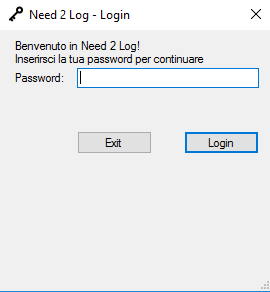
\includegraphics[scale=1]{immagini/test/testUC1_1.png}
							\end{center}
						\begin{figure}[!h]
								\caption{Prima screenshot del test per UC1}
							\end{figure}}
					\item[] {
						\begin{center}
							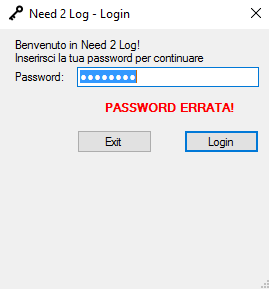
\includegraphics[scale=1]{immagini/test/testUC1_2.png}
							\end{center}
						\begin{figure}[!h]
								\caption{Seconda screenshot del test per UC1}
							\end{figure}}
					\item[] {
						\begin{center}
							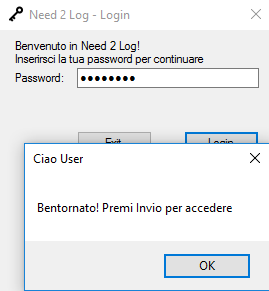
\includegraphics[scale=1]{immagini/test/testUC1_3.png}
							\end{center}
						\begin{figure}[!h]
								\caption{Terza screenshot del test per UC1}
							\end{figure}}
					\item[] {
						\begin{center}
							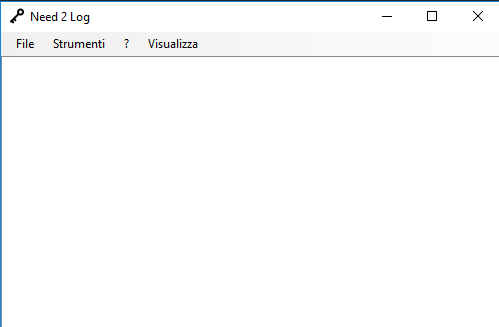
\includegraphics[scale=1]{immagini/test/testUC1_4.png}
							\end{center}
						\begin{figure}[!h]
								\caption{Quarta screenshot del test per UC1}
							\end{figure}}
					\end{itemize}
			\newpage
			\subsection{Test UC2 - New account}
				\begin{itemize}
					\item[] {
						\begin{center}
							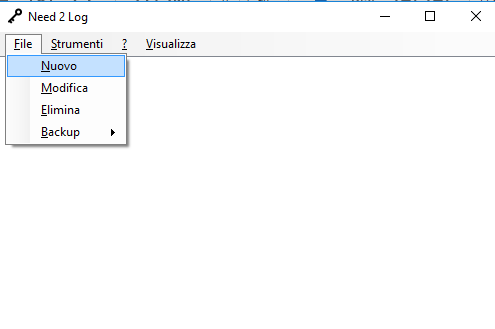
\includegraphics[scale=1]{immagini/test/testUC2_1.png}
							\end{center}
						\begin{figure}[!h]
								\caption{Prima screenshot del test per UC2}
							\end{figure}}
					\item[] {
						\begin{center}
							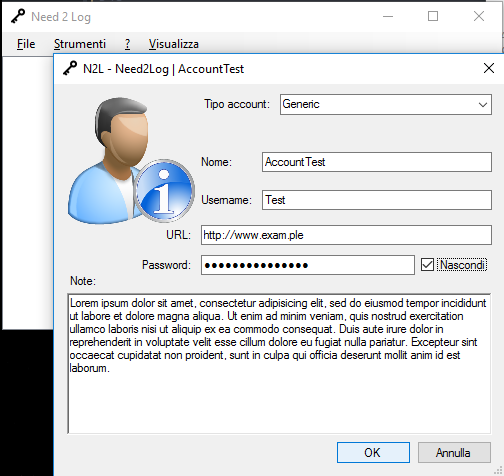
\includegraphics[scale=1]{immagini/test/testUC2_2.png}
							\end{center}
						\begin{figure}[!h]
								\caption{Seconda screenshot del test per UC2}
							\end{figure}}
					\item[] {
						\begin{center}
							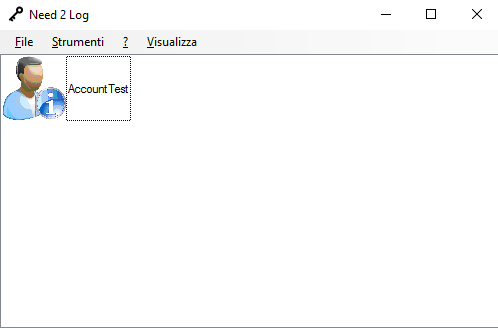
\includegraphics[scale=1]{immagini/test/testUC2_3.png}
							\end{center}
						\begin{figure}[!h]
								\caption{Terza screenshot del test per UC2}
							\end{figure}}
					\end{itemize}
			\newpage
			\subsection{Test UC4 - Delete account}
				\begin{itemize}
					\item[] {
						\begin{center}
							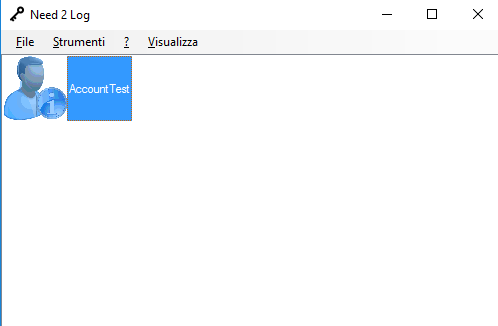
\includegraphics[scale=1]{immagini/test/testUC4_1.png}
							\end{center}
						\begin{figure}[!h]
								\caption{Prima screenshot del test per UC4}
							\end{figure}}
					\item[] {
						\begin{center}
							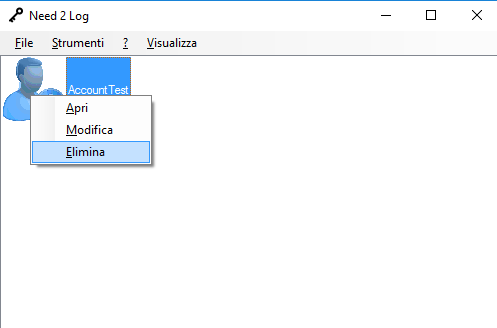
\includegraphics[scale=1]{immagini/test/testUC4_2.png}
							\end{center}
						\begin{figure}[!h]
								\caption{Seconda screenshot del test per UC4}
							\end{figure}}
					\item[] {
						\begin{center}
							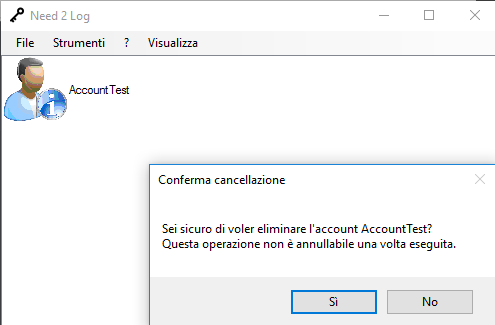
\includegraphics[scale=1]{immagini/test/testUC4_3.png}
							\end{center}
						\begin{figure}[!h]
								\caption{Terza screenshot del test per UC4}
							\end{figure}}
					\item[] {
						\begin{center}
							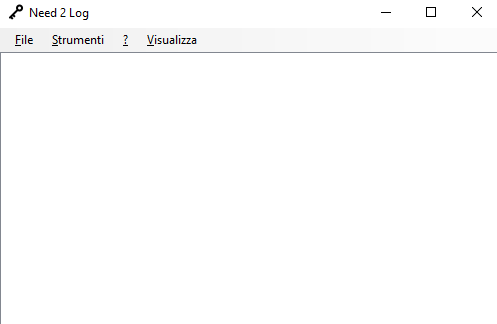
\includegraphics[scale=1]{immagini/test/testUC4_4.png}
							\end{center}
						\begin{figure}[!h]
								\caption{Quarta screenshot del test per UC4}
							\end{figure}}
					\end{itemize}
			\newpage
			\subsection{Test UC5 - Show account}
				\begin{itemize}
					\item[] {
						\begin{center}
							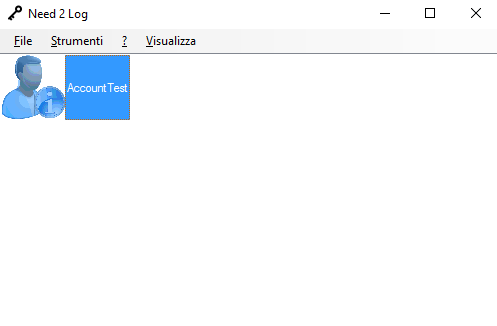
\includegraphics[scale=1]{immagini/test/testUC5_1.png}
							\end{center}
						\begin{figure}[!h]
								\caption{Prima screenshot del test per UC5}
							\end{figure}}
					\item[] {
						\begin{center}
							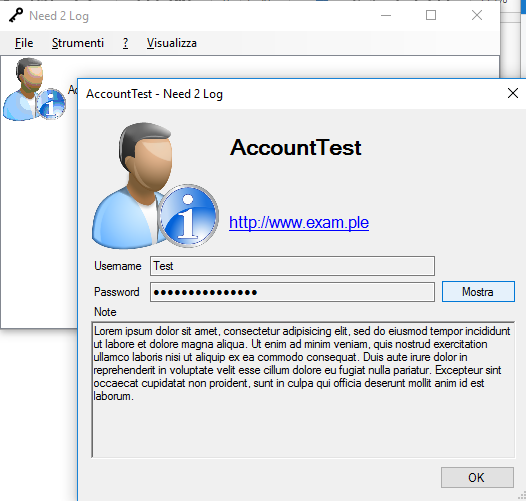
\includegraphics[scale=1]{immagini/test/testUC5_2.png}
							\end{center}
						\begin{figure}[!h]
								\caption{Seconda screenshot del test per UC5}
							\end{figure}}
					\item[] {
						\begin{center}
							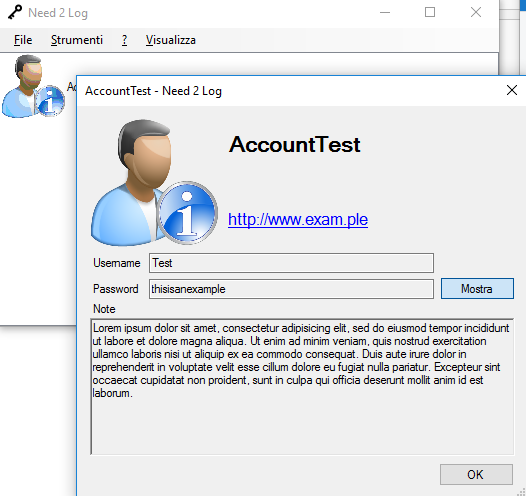
\includegraphics[scale=1]{immagini/test/testUC5_3.png}
							\end{center}
						\begin{figure}[!h]
								\caption{Terza screenshot del test per UC5}
							\end{figure}}
					\end{itemize}
\newpage
\chapter{Compilazione ed esecuzione} %
	\section{Requisiti di sistema}
		Poiché l’applicazione non risulta onerosa in termini di potenza
			computazionale e di memoria occupata, i requisiti minimi coincidono
			con quelli di tutte le applicazioni sviluppate con il framework .NET.
		\subsection{Requisiti minimi}
			\begin{itemize}
				\item Processore 1 GHz o superiore con architettura x86 o x86\_64
				\item 512 Mb di memoria principale
				\item 600 Mb di spazio su disco per sistemi a 32 bit
				\item 1.5 Gb di spazio su disco per sistemi a 64 bit
				\item Sistema operativo Microsoft Windows 7 SP1 o successivo
				\item Piattaforma .NET 4.5.2 installata.
			\end{itemize}
		\subsection{Requisiti consigliati}
			\begin{itemize}
				\item Processore 1 GHz o superiore con architettura x86 o x86\_64
				\item 512 Mb di memoria principale
				\item 850 Mb di spazio su disco per sistemi a 32 bit
				\item 2 Gb di spazio su disco per sistemi a 64 bit
				\item Sistema operativo Microsoft Windows 7 SP1 o
					successivo per ambienti desktop
				\item Sistema operativo Microsoft Windows Server 2008 SP2 o
					successivo per ambienti server
				\item Piattaforma .NET 4.6 installata.
			\end{itemize}
			Si sono effettuati test su varie macchine, confermando empiricamente che
				i requisiti sopra descritti risultano sufficienti all’esecuzione senza
				crash o rallentamenti.
  \section{Compilazione con Visual Studio}
		\begin{enumerate}
			\item Navigare fino alla cartella {\itshape Need2Log} ed accedervi;
			\item Avviare il file {\itshape N2L.sln} con {\itshape Visual Studio};
			\item Verificare che la configurazione sia impostata su {\itshape Release};
			\item Selezionare la voce di menù {\itshape Compila}{\rightarrow}{\itshape Compila Soluzione}
			\end{enumerate}
  \section{Esecuzione}
    \begin{enumerate}
    	\item Dalla cartella {\itshape Need2Log}, navigare nel percorso {\itshape Need2Log/N2L-Need\_2\_Log/bin/Release}
			\item Fare doppio click sul file eseguibile "{\itshape Need 2 Log.exe}"
    	\end{enumerate}
		L'applicativo è stato testato su vari elaboratori con differenti sistemi
			operativi e differenti configurazioni hardware per verificare se il
			comportamento del programma mutasse (anche a livello di performance),
			ma non sono state riscontrate differenze nel funzionamento.\\
			Nello specifico, l'applicazione è stata testata su:
		\begin{table}[h]
			\centering
			\begin{tabular}{|c|c|c|c|}
				\hline
				\textbf{Sistema operativo} & \textbf{RAM (GB)} & \textbf{CORE} & \textbf{Architettura}\\ \hline
				Windows 7 & 4 GB & 2 Core & 64 bit\\ \hline
				Windows 8.1 & 8 GB & 4 Core & 64 bit\\ \hline
				Windows 10 & 5 GB & 4 Core & 64 bit\\ \hline
				Windows 10 & 8 GB & 8 Core & 64 bit\\
				\hline
				\end{tabular}
			\caption{Specifiche delle macchine su cui il programma è stato eseguito}
			\label{tab:tabellaTest}
			\end{table}
\end{document}
